\documentclass{article}
\usepackage[utf8]{inputenc}
\usepackage[danish]{babel}
\usepackage{graphicx}
\usepackage{amsmath}
\usepackage[document]{ragged2e}
\usepackage{hyperref}
\usepackage{listings}
\usepackage{color}
\usepackage{tikz-qtree}
\usepackage[T1]{fontenc}
\hypersetup{
	colorlinks,
	citecolor=black,
	filecolor=black,
	linkcolor=black,
	urlcolor=black
}

\definecolor{mygreen}{rgb}{0,0.6,0}
\definecolor{mygray}{rgb}{0.5,0.5,0.5}
\definecolor{mymauve}{rgb}{0.58,0,0.82}

\lstset{ %
	backgroundcolor=\color{white},   % choose the background color
	basicstyle=\footnotesize,        % size of fonts used for the code
	breaklines=true,                 % automatic line breaking only at whitespace
	captionpos=b,                    % sets the caption-position to bottom
	commentstyle=\color{mygreen},    % comment style
	escapeinside={\%*}{*)},          % if you want to add LaTeX within your code
	keywordstyle=\color{blue},       % keyword style
	stringstyle=\color{mymauve},     % string literal style
	numbers=left,
	stepnumber=1, 
	tabsize=2,   
	firstnumber=1,
	numberfirstline=true,
	frame=single
}

\title{Dispositioner - dProg2 Eksamen}
\author{Martin Nørskov Jensen \\ 201610882}

\begin{document}
	
\maketitle
\newpage

\tableofcontents

\newpage


\section{Recursive methods and recursive data structures}

\subsection{Rekursive metoder}
\begin{itemize}
	\item Rekursive metoder er metoder der kalder sig selv.
	\item Der findes ofte en mere kompliceret version af den rekursive metode, som ikke er rekursiv og derfor hurtigere. 
	\item Rekursive metoder kan blandt andet bruges til at udregne Fibonacci tal
	\begin{itemize}
		\item Fibonacci er en talfølge, hvor det n'te fibonacci tal er lige med de 2 foregående tal lagt sammen
		\item Når man beskriver en rekursive metode skriver man det således, her er Fibonacci funktionen skrevet op:
	 	\begin{equation}
		F_n =
		\begin{cases}
			\mbox{1} & \mbox{n=0,1} \\
			\mbox{$F_{n-1}+F_{n-2}$} & \mbox{n>1} \\
		\end{cases}
		\end{equation}
		\item En Fibonacci funktion ser således ud i Java:
\begin{lstlisting}[language=java]
public long fib(int n){
	if(n <= 1) return 1;
	else return fib(n-1) + fib(n-2);
}
\end{lstlisting}
	\item Når man kalder fib(4), skaber den følgende træstruktur af funktionskald: \\
	\Tree [.fib(4) [.fib(3) [.fib(2) [.fib(1) ] [.fib(0) ] ] [.fib(1) ] ] [.fib(2) [.(fib(1) ] [.fib(0) ] ] ]
	\item Som man kan se på denne metode bliver funktionen kaldt med den samme værdi flere gange. 
	\item Man kan også skrive funktionen, så den bruger iteration i stedet for rekursion, så kommer den til at se således ud:
\begin{lstlisting}[language=java]
public long fib(int n){
	long firstNumb = 0L;
	long secondNumb  = 1L;
	for(int i = 0; i<n; i++){
		long result = 0L;
		result = firstNumb + secondNumb;
		firstNumb = secondNumb;
		secondNumb = result;		
	}
	
	return secondNumb;
}
\end{lstlisting}	
	\end{itemize} 
	\item Når man laver en rekursiv funktion er det vigtigt, med et stop kriterie ellers stopper funktionen aldrig.
	\item Man kan også bruge rekursive kald til at tegne fraktaler. En kochLine er et godt eksempel på dette:
	\begin{figure}[ht!]
		\centering
		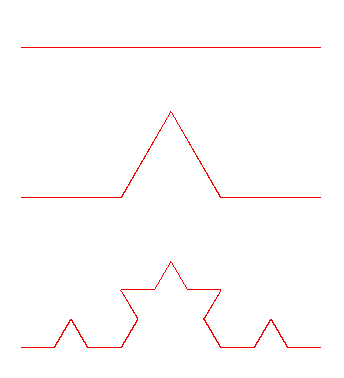
\includegraphics[width=100mm]{img/kockLine.png}
		\caption{KochLinje af 1, 2 og 3 orden  \label{KochLinje}}
	\end{figure}

		\item Koden for denne kurve ser således ud:
\begin{lstlisting}[language=java]
private void kochLine(int order, double len) {
	if (order == 0) c.move(len);
	else if (order > 0) {
		kochLine(order-1,len/3); c.turn(-60);
		kochLine(order-1,len/3); c.turn(120);
		kochLine(order-1,len/3); c.turn(-60);
		kochLine(order-1,len/3);
	}
}
\end{lstlisting}		
	\item Denne funktion bruger c, som er et Crayon objekt, der bruges til at tegne linjen. move(len) tegner en linje af længden len. C.turn(x) roter crayon x grader
	\item Denne funktion vil være meget mere besværlig at lave en ikke rekursiv metode til, da den hurtig bliver meget kompliceret i større ordener.

\end{itemize}

\subsection{Rekursive datastrukturer}
\begin{itemize}
	\item Filsystemer er et eksempel på en rekursiv datastruktur.
	\item Rekursive datastruktur kan beskrives, som en rekursiv træstruktur.
	\begin{itemize}
		\item En rekursiv datastruktur er et eksempel på brug af Composite pattern, hvor et Composite objekt både kan indeholde simple objekter (Leaf) og andre Composite objektor (Node)
	\end{itemize}
		\begin{figure}[ht!]
		\centering
		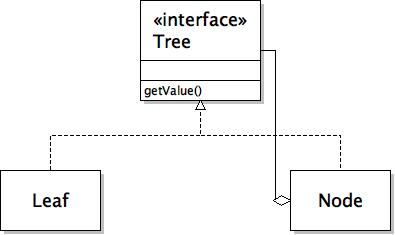
\includegraphics[width=100mm]{img/rekursiveComposite.jpeg}
		\caption{En rekursiv træstruktur \label{UMLrekursiv}}
	\end{figure}
	\item Man kan omskrive aritmetiske udtryk til rekursive træstrukturer.
	\newpage
	\begin{center}
		\Tree [.\node[draw,circle]{+};
		[.\node[draw,circle]{6};] [.\node[draw,circle]{-}; [.\node[draw,circle]{*}; 
		[.\node[draw,circle]{5};] [.\node[draw,circle]{10};] ] 
		[.\node[draw,circle]{7};]] ] 
		\\
		\bigskip
		Eksempel på rekursiv træstruktur over det aritmetiske udtryk: $6+((5*10)-7)$
	\end{center}
	
	\item Man kan så ud fra dette lave en rekursiv træstruktur, hvor Leaf er et enkelt tal og hvor Node består af en operator og en højre side og venstre side. 
	\item Man kan så bruge funktionen \textit{getValue()} for at evaluere udtrykkene
\end{itemize}

\subsection{Visitor Pattern}
\begin{itemize}
	\item Problem
	\begin{enumerate}
		\item En objekt struktur indholder flere forskellige slags element typer og man vil gerne udføre forskellige operation afhængig af objekt typen
		\item Det skal være muligt at udvide antal operationer over tid
		\item Antallet af element klasser er fastsat
	\end{enumerate}
	\item Løsning
	\begin{enumerate}
		\item Definere en visitor interface type, der har metoder til at besøge hver enkelt element type.
		\item Hver element type har en accept metode, der starter den tilsvarende metode på det pågældende objekt
		\item Hvis man vil implementere en ny operation, skal man lave en klasse, som implementere visitor interface typen og som har en operation for hver element type.  
	\end{enumerate}
	\item UML Diagram
	\newpage
	\begin{figure}[ht!]
		\centering
		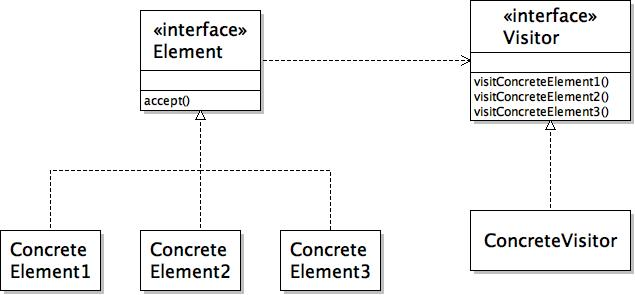
\includegraphics[width=100mm]{img/visitorUML.jpeg}
		\caption{Visitor Pattern  \label{UMLvisitor}}
	\end{figure}
	
	\item Eksempel:
	\begin{itemize}
		\item Filsystem:
		\begin{itemize}
			\item \textbf{Element:} FileSystemNode
			\item \textbf{ConcreteElement:} FileNode, DirectoryNode
			\item \textbf{Visitor:} FileSystemVisitor
			\item \textbf{ConcreteVisitor:} PrintVisitor
		\end{itemize}
	\end{itemize}
\end{itemize}

\newpage
\subsection{Disposition}
\begin{enumerate}
	
	\item Hvad er rekursive metoder?
	\begin{itemize}
		\item Fordele: nemmere at implementerer
		\item Ulemper: Ikke den mest effektive metode
	\end{itemize}
	
	\item Rekursive metoder
	\begin{itemize}
		\item Fibonacci sekvens
		\item Fraktaler
		\item Eksempler på rekursive metoder?
		
	\end{itemize}
	\item Rekursive datastrukturer
	\begin{itemize}
		\item Hvad er en rekursive datastruktur?
		\item Rekursive træer
		\item Aritmetiske udtryk som rekursive træer. 
	\end{itemize}

	\item{Visitor Pattern}
	\begin{itemize}
		\item Problem
		\item Løsning
		\item UML Diagram
		\item Filsystem Eksempel
	\end{itemize}
	
\end{enumerate}

\newpage

\section{Polymorphism and Interfaces}
Polymorfi er defineret som: \textit{"evnen til at vælge forskellig metoder med hensyn til objekt typen"}. Dette betyder, at programmøren til en metode, som gøre brug af polymorfi ikke nødvendigvis kender implentationen af de klasser som bliver brugt. Men kun nogle konkrete metoder i de klasser. 

\subsection{Interface}
\begin{itemize}
	\item Et interface har ingen instanceret metoder
	\item Det er den, som implementere et interfaces job at implementer alle metoderne
	\item Et interface kan ikke have nogle feltvariabler, den kan kun have konstanter. 
	\item For at implementere et interface bruges nøgleordet \textit{implements} i Java
	\item Eksempel:
	\begin{figure}[ht!]
		\centering
		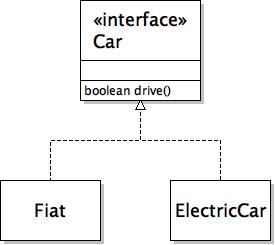
\includegraphics[width=80mm]{img/UMLiconeksempel.jpeg}
		\caption{UML diagram over eksemplet	\label{UMLiconeksempel}}
	\end{figure}
\begin{lstlisting}[language=java]
public interface Car{
	boolean drive(double distance));
	...
}
\end{lstlisting}
\begin{lstlisting}[language=java]
public class Fiat implements Car{
	private double _fuel;
	
	public Fiat(double fuel){
		_fuel = fuel;
	}
	
	public boolean drive(double distance){
		if(fuel>= distance*0.10){
			fuel-distance*0.10;
			return true;
		}
		return false;
	}
	...
}
\end{lstlisting}
\begin{lstlisting}[language=java]
public class Fiat implements Car{
	private double _charge;
	
	public Fiat(double charge){
		_charge = charge;
	}
	
	public boolean drive(double distance){
		if(fuel>= distance*0.01){
			charge-distance*0.10;
			return true;
		}
		return false;
	}
	...
}
\end{lstlisting}
\end{itemize}

\subsection{Polymorfi}
\begin{itemize}
	\item Polymorfi bruges ofte, når en metode skal bruges på mange forskellige slags objekter som minder om hinanden. Dette gøres ved bruges af \textbf{Interfaces} og/eller \textbf{Abstrakte klasser} 
	\item En klasse har to typer, dens statiske type og dens dynamiske type.
	\begin{itemize}
		\item En klasses dynamiske type er den type, som klasse faktisk er.
		\item En klasses statiske type er den type, som klassen er defineret ud fra.
		\item Hvis du kalder en metode på en klasse. Er det klassens dynamiske type, som afgør hvilken metode man skal kalde
		\item Hvis man bruger en klasse i en anden klasses metode, er det den statiske type, som afgør hvilken metode der skal kaldes.  
	\end{itemize}
\end{itemize}

\subsection{Nedarvning}
\begin{itemize}
	\item Man taler om nedarvning, når man laver subklasser af en bestemt klasse, som så bliver kaldt en superklasse.
	\item En subklasse er en mere specialiseret version af dens superklasse
	\item En subklasse arver alle superklassens metoder og feltvariabler, men kan ikke tilgå dem direkte
	\item Man bruger \textit{"extends"} nøgleordet til at udvide klasser i Java
	\item Når man laver subklasser af en klasse er det vigtigt at bruge \textit{"is a testen"}, for at finde ud af om det giver mening at lave en subklasse af et objekt.
	\begin{itemize}
		\item I \textit{"is-a-testen"} spørger man om <subklassen> is a <superklassen>
	\end{itemize}
	\item Når man \textbf{overrider} en metode i Java betyder det, at man overskriver superklassens version af den pågældende metode
	\begin{itemize}
		\item Når man overrider en metode, må man ikke lave preconditions stærkere,
		\item Man skal også sørger for at overhold \textbf{Lisskovs Substitutions Princip}, som går ud på, at en subklasse af en metode skal kunne bruges samme steder som dens superklasse 
		\item Man skal også sørger for at parameterne er de samme eller overloader man
		\item Returtypen skal enten være den samme type eller en subtype af den pågældende type 
	\end{itemize}
	\item Når man \textbf{overloader} betyder det, at man laver en metode med samme navn som en anden metode dog med anden returtype og/eller parameter.
	\item Polymorfi gør at uanset hvad den statiske dynamiske klasse er, så bliver den overridet metode kaldt	
	\item Når man laver en subklasse kan man overskrive superklassen metoder med mere specialiseret metoder. Men hvis man ønsker at kalde superklassen metoder bruger \textit{"super"} nøgleordet i Java
	\item For at en subklasse, skal kunne tilgå superklassens metoder bruger man nøgle ordet \textit{protected}, hvis man ikke vil lave metoden \textit{public}.
\end{itemize}

\subsection{Abstrakt Klasse}
\begin{itemize}
	\item En abstrakt klasse er en klasse, som man ikke kan lave objekter af.
	\item I en abstrakt klasse har oftest nogle uimplementeret metoder 
	\item En abstrakt klasse kan modsat et interface godt have feltvariabler. 
	\begin{itemize}
		\item For at udvide en abstrakt klasse i Java bruges nøgleordet \textit{extends}
		\item For at lave en abstrakt klasse i Java bruges nøgleordet \textit{abstract} 
	\end{itemize}
	\item Abstrakte klasser bruges ofte i forbindelse med Interfaces, hvis en del af implantationen er ens for en eller flere klasser.
	\item Når man fjerne gentagelser i ens kode vha. abstrakte klasser kaldes det for \textbf{Refaktorisering}
	\begin{figure}[ht!]
		\centering
		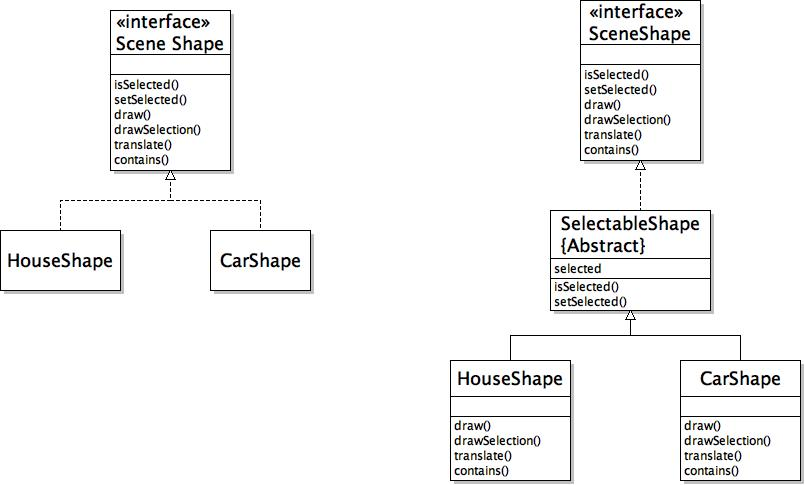
\includegraphics[width=100mm]{img/UMLabstract.jpeg}
		\caption{Refaktorerings Eksempel  \label{UMLinterface}}
	\end{figure}
	\item Forskellen på Interface og Abstrakt klasse:
	\begin{enumerate}
		\item Et \textbf{Interface} har kun ikke instantieret metoder, mens en \textbf{Abstrakt klasse} kan have måde instantieret og ikke instantieret metoder 
		\item En \textbf{Abstrakt klasse} kan godt implementer Interfaces og udvide andre klasser, et \textbf{Interface} ikke kan gøre nogle af delene
		\item Et \textbf{Interface} kan kun have konstanter, mens en \textbf{Abstrakt klasse} kan have både feltvariabler og konstanter
		\item Man kan implementere flere forskellige Interfaces, men man kan kun udvide en Abstrakt klasse.
	\end{enumerate}
\end{itemize}

\newpage
\subsection{Disposition}
\begin{enumerate}
	\item Interfaces
	\begin{itemize}
		\item Hvad er et interface?
		\item Interface Eksempel 
	\end{itemize}
	\item Polymorfi 
	\begin{itemize}
		\item Hvad er polymorfi?
		\item Overriding og overloading (Liskovs Substitions Princip)
		\item Statikstype overfor dynamisktype
		\item Interfaces og abstrakte klasser i forbindelse med polymorfi
		\item JOptionPane Eksempel
	\end{itemize}
		\item Nedarvning 
	\begin{itemize}
		\item Superklasser og subklasser
		\item \textit{"is a testen"}
	\end{itemize}
		\item Abstrakte klasser
		\begin{itemize}
			\item Hvad er en abstrakt klasse
			\item Forskellen på en abstrakt klasse og et interface
		\end{itemize}
\end{enumerate}
\newpage

\section{Design Patterns}
Et design mønster inden for programmering er en måde at løse et konkret problem på. I et design mønster bliver der stillet et problem i nogle punkter og så kommer der et forslag til hvordan man kan løse det vha. et UML diagram. 

\subsection{Composite Pattern}
\begin{itemize}
	\item Problem
	\begin{enumerate}
		\item Få composite objekter til at indeholder måde andre af samme type objekter eller en primitiv form
		\item Primitive objekter skal kunne blive kombineret sammen med composite objekter i et composite objekt
		\item Et composite objekt skal blive behandlet som et primitivt objekt.
	\end{enumerate}
	\item Løsning
	\begin{enumerate}
		\item Definere et interface type, som er en abstraktion for primitive objekter
		\item Et composite objekt indeholder en samling af primitive objekter
		\item Både composite objekter og primitive objekter implementerer interfacet. 
		\item Når man implementere en metode fra interface typen, skal composite objekterne bruge metoden på dens primitive objekter og kombinerer resultatet.
	\end{enumerate}
	\item UML Diagram
	\begin{figure}[ht!]
		\centering
		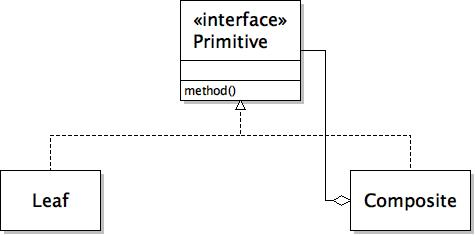
\includegraphics[width=100mm]{img/compositeUML.jpeg}
		\caption{Composite Pattern  \label{UMLDesign1}}
	\end{figure}
	\item Eksempel
	\begin{itemize}
		\item Java Layout
		\begin{itemize}
			\item \textbf{Primitive:} Component 
			\item \textbf{Leaf:} Et Component uden børn såsom jButton
			\item \textbf{Composite: } En container fx. jPanel
			\item \textbf{method():} Fx. \textit{getPreferedSize()} 
		\end{itemize}
		\item FilSystem
		\begin{itemize}
			\item \textbf{Primitive:} FileSystemObjekt 
			\item \textbf{Leaf:} File
			\item \textbf{Composite:} Folder 
			\item \textbf{method():} Fx. \textit{getSize()}
		\end{itemize}
	\end{itemize}
\end{itemize}

\subsection{Template Method Pattern}
	\begin{itemize}
		\item Problem
		\begin{enumerate}
			\item En algoritme kan bruges til flere forskellig klasser
			\item Algoritmen kan blive delt ned til flere primitive operationer, hvor de primitive operationer er forskellig fra klasse til klasse
			\item Ordren af de primitive operationer har ikke noget med klassetypen at gøre
		\end{enumerate}
		\item Løsning
		\begin{enumerate}
			\item Definere en abstrakt klasse, som har en metode for algorimen og abstrakte metoder for de primitive operationer
			\item Implementer algorimen, så den kalder de primitive operationer i den rigtige rækkefølge
			\item Enten lad vær med at definere de primitive operationer i superklassen eller lav en god default implementation
			\item Alle subklasser definere de primitive operationer og ikke algoritmen.  
		\end{enumerate}
		\newpage
		\item UML Diagram
		\begin{figure}[ht!]
			\centering
			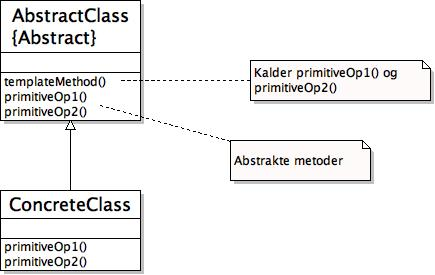
\includegraphics[width=100mm]{img/templateUML.jpeg}
			\caption{Template Method Pattern  \label{UMLDesign3}}
		\end{figure}
		\item Eksempel
		\begin{itemize}
			\item Carnivore eksempelet fra review opgaver
			\begin{itemize}
				\item \textbf{AbstractClass:} Carnivore
				\item \textbf{templateMethod():} live()
				\item \textbf{primitiveOp():} hunt(), eat(), rest()
				\item \textbf{ConcreteClass:} Cat 
				\item \textbf{Kode Eksempel:}
\begin{lstlisting}[language=java]
public abstract class Animal {
	private int energyLevel;
	...
	public abstract void live();

}    

\end{lstlisting}

\begin{lstlisting}[language=java]
public abstract class Carnivore extends Animal {
	private int lengthOfLife;

	public Carnivore(int cycles) {
		super();
		lengthOfLife = cycles;
	}
	
	public void live() {
		eat();
		for (int i = 1; i <= lengthOfLife; i++) {
			hunt();
			eat();
			rest();
		}
	}
	
	public abstract void hunt();
	public abstract void eat();
	public abstract void rest();
}
\end{lstlisting}

\begin{lstlisting}[language=java]
public class Cat extends Carnivore {
	public Cat() {
		super(50);
	}
	
	public void hunt() {
		consumeEnergy(10);
	}
	
	public void eat() {
		storeEnergy(13);
	}
	
	public void rest() {
		consumeEnergy(2);
	}
}
\end{lstlisting}					
			\end{itemize}
		\end{itemize}
	\end{itemize}

\subsection{Observer Pattern}
\begin{itemize}
	\item Problem
	\begin{enumerate}
		\item Et objekt er kilde til en begivenheden (subjekt)
		\item En eller flere andre objekter er interesseret i hvornår denne begivenhed sker (observer)
	\end{enumerate}
	\item Løsning
	\begin{enumerate}
		\item Definere en Interface type som alle "observer" skal implementere. 
		\item Alle subjekter inderholder en samling af observere objekts 
		\item Subjekt klassen indeholder en methode til at tilføje observers
		\item Når der sker et event skal alle observere informeres
	\end{enumerate}
	\item UML Diagram
	\begin{figure}[ht!]
		\centering
		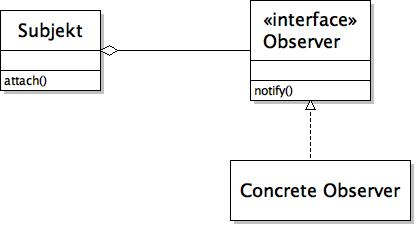
\includegraphics[width=100mm]{img/observerUML.jpeg}
		\caption{Observer Pattern  \label{UMLDesign2}}
	\end{figure}
	\item Eksempel
	\begin{itemize}
		\item jButton
		\begin{itemize}
			\item \textbf{Subjekt:} jButton
			\item \textbf{attach():} addActionListener()
			\item \textbf{Observer:} ActionListener 
			\item \textbf{notify():} actionPerformed()
			\item \textbf{Concrete Observer:} En klasse, som implementer ActionListener interfacet 
		\end{itemize}
	\end{itemize}
\end{itemize}


\newpage
\subsection{Disposition}
\begin{enumerate}
	\item Design Pattern
	\begin{itemize}
		\item Hvad er et design mønster?
	\end{itemize}
	\item Composite Pattern
	\begin{itemize}
		\item Problem
		\item Løsning
		\item UML Diagram
		\item Filsystem og Layout Eksempel
	\end{itemize}
	\item Observer Pattern 
	\begin{itemize}
		\item Problem
		\item Løsning
		\item UML Diagram
		\item jButton Eksempel
	\end{itemize}
	\item Template Method Pattern 
	\begin{itemize}
		\item Problem
		\item Løsning
		\item UML Diagram
		\item Carnivorer Eksempel
	\end{itemize}
\end{enumerate}

\newpage
\section{Inheritance and Abstract Classes}

\subsection{Abstract Klasse}
\begin{itemize}
	\item En abstrakt klasse er en klasse, som man ikke kan lave objekter af.
	\item I en abstrakt klasse har oftest nogle uimplementeret metoder 
	\item En abstrakt klasse kan modsat et interface godt have feltvariabler. 
	\begin{itemize}
		\item For at udvide en abstrakt klasse i Java bruges nøgleordet \textit{extends}
		\item For at lave en abstrakt klasse i Java bruges nøgleordet \textit{abstract} 
	\end{itemize}
	\item Abstrakte klasser bruges ofte i forbindelse med Interfaces, hvis en del af implantationen er ens for en eller flere klasser.
	\item Når man fjerne gentagelser i ens kode vha. abstrakte klasser kaldes det for \textbf{Refaktorisering}
	\begin{figure}[ht!]
		\centering
		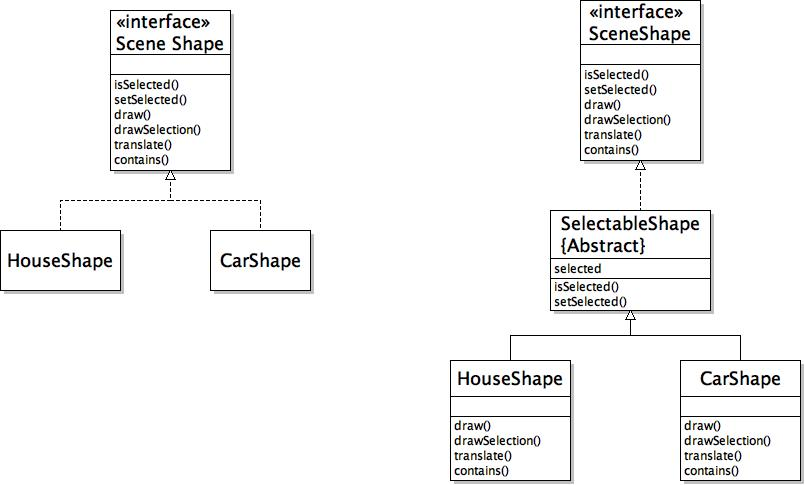
\includegraphics[width=100mm]{img/UMLabstract.jpeg}
		\caption{Refaktorerings Eksempel  \label{UMLAbstract1}}
	\end{figure}
\end{itemize}

\subsection{Nedarvning}
\begin{itemize}
	\item Man taler om nedarvning, når man laver subklasser af en bestemt klasse, som så bliver kaldt en superklasse.
	\item En subklasse er en mere specialiseret version af dens superklasse
	\item En subklasse arver alle superklassens metoder og feltvariabler, men kan ikke tilgå dem direkte
		\item Man bruger \textit{"extends"} nøgleordet til at udvide klasser i Java
	\item Når man laver subklasser af en klasse er det vigtigt at bruge \textit{"is a testen"}, for at finde ud af om det giver mening at lave en subklasse af et objekt.
	\begin{itemize}
		\item I \textit{"is-a-testen"} spørger man om <subklassen> is a <superklassen>
	\end{itemize}
	\item Når man \textbf{overrider} en metode i Java betyder det, at man overskriver superklassens version af den pågældende metode
	\begin{itemize}
		\item Når man overrider en metode, må man ikke lave preconditions stærkere,
		\item Man skal også sørger for at overhold \textbf{Lisskovs Substitutions Princip}, som går ud på, at en subklasse af en metode skal kunne bruges samme steder som dens superklasse 
		\item Man skal også sørger for at parameterne er de samme eller overloader man
		\item Returtypen skal enten være den samme type eller en subtype af den pågældende type 
	\end{itemize}
	\item Når man \textbf{overloader} betyder det, at man laver en metode med samme navn som en anden metode dog med anden returtype og/eller parameter.
	\item Polymorfi gør at uanset hvad den statiske dynamiske klasse er, så bliver den overridet metode kaldt
	\item Når man laver en subklasse kan man overskrive superklassen metoder med mere specialiseret metoder. Men hvis man ønsker at kalde superklassen metoder bruger \textit{"super"} nøgleordet i Java
	\item For at en subklasse, skal kunne tilgå superklassens metoder bruger man nøgle ordet \textit{protected}, hvis man ikke vil lave metoden \textit{public}.
\end{itemize}

\subsection{Polymorfi}
\begin{itemize}
	\item Polymorfi bruges ofte, når en metode skal bruges på mange forskellige slags objekter som minder om hinanden. Dette gøres ved bruges af \textbf{Interfaces} og/eller \textbf{Abstrakte klasser} 
	\item En klasse har to typer, dens statiske type og dens dynamiske type.
	\begin{itemize}
		\item En klasses dynamiske type er den type, som klasse faktisk er.
		\item En klasses statiske type er den type, som klassen er defineret ud fra.
		\item Hvis du kalder en metode på en klasse. Er det klassens dynamiske type, som afgør hvilken metode man skal kalde
		\item Hvis man bruger en klasse i en anden klasses metode, er det den statiske type, som afgør hvilken metode der skal kaldes.  
	\end{itemize}
	\item Polymorfi gør at uanset hvad den statiske dynamiske klasse er, så bliver den overridet metode kaldt
	\item Et eksempel på en metode som bruger polymorfi er klassen JOptionPanes metode showMessageDialog, som blandt andet tager en Icon type, som parameter:	
\end{itemize}

\subsection{Interface}
\begin{itemize}
	\item Et interface har ingen instanceret metoder
	\item Det er den, som implementere et interfaces job at implementer alle metoderne
	\item Et interface kan ikke have nogle feltvariabler, den kan kun have konstanter. 
	\item For at implementere et interface bruges nøgleordet \textit{implements} i Java
	\item Forskel på en abstrakt klasse og et interface:
	\begin{enumerate}
		\item Et \textbf{Interface} har kun ikke instantieret metoder, mens en \textbf{Abstrakt klasse} kan have måde instantieret og ikke instantieret metoder 
		\item En \textbf{Abstrakt klasse} kan godt implementer Interfaces og udvide andre klasser, et \textbf{Interface} ikke kan gøre nogle af delene
		\item Et \textbf{Interface} kan kun have konstanter, mens en \textbf{Abstrakt klasse} kan have både feltvariabler og konstanter
		\item Man kan implementere flere forskellige Interfaces, men man kan kun udvide en Abstrakt klasse.
	\end{enumerate}
\end{itemize}



\newpage
\subsection{Disposition}
\begin{enumerate}
	\item Abstrakte klasser
	\begin{itemize}
		\item Hvad er en abstrakt klasse?
		\item Eksempel på brug af en abstrakt klasse
	\end{itemize}
	\item Super- og subklasser 
	\begin{itemize}
		\item Hvad er Super- og subklasser
		\item Nedarvning
		\item is-a-testen
	\end{itemize}
	\item Overridning / Overloading
	\begin{itemize}
		\item Overriding vs overloading
		\item Lisskovs substitutions princip
	\end{itemize}
	\item Statiske / Dynamiske typer 
	\begin{itemize}
		\item Hvad er en statiske og dynamisk klasse
		\item Overloading Eksempel
	\end{itemize}
	
\end{enumerate}
\newpage

\section{Exceptions and Files}

\subsection{Exceptions}
\begin{itemize}
	\item En exception er en subklasse af Throwable
	\item En exception bliver smidt, når der er sket en form for fejl i programmet.
	\item For at smide en exception bruger man nøgleordet throw også exception typen:
\begin{lstlisting}[language=java]
...
	throw new NullPointerException("besked");
...
\end{lstlisting}
	\item Sådan ser UML-diagrammet ud for en Exceptions:
	\begin{figure}[ht!]
		\centering
		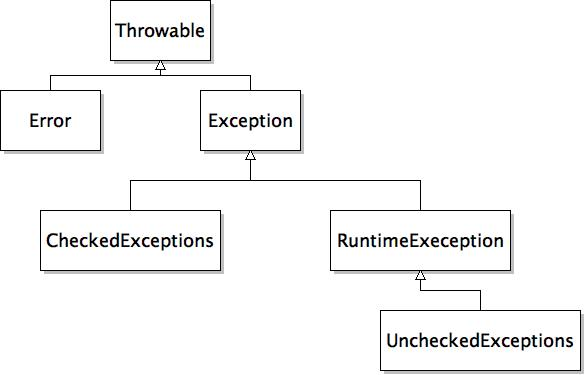
\includegraphics[width=100mm]{img/exceptionsUML.jpeg}
		\caption{Exceptions UML \label{UMLExceptions1}}
	\end{figure}
	\item Exception håndtering er, hvordan er programmør håndter exceptions (Defensive programming)
	\begin{itemize}
		\item Det er en programmørs job at sørger for at Exceptions bliver behandlet ordentligt. 
	\end{itemize}
	\item For at fange en exception bruger man en \textit{try-catch block}, som ser således:
\begin{lstlisting}[language=java]
public class Test{
	public static void main(String[] args){
		try{
			String name = args[0];
			System.out.println(name);
		}catch(ArrayIndexOutOfBoundsException e){
			System.out.println("Please supply your name!")M
		}
	}
}
\end{lstlisting}
	\item Man kan også bruge en finally clause efter catch, som sikre sig at den del af koden altid bliver eksekveret.
	\begin{itemize}
		\item En finally clause bliver altid eksekveret også selvom, der har været en return kald.
		\item Den bliver også eksekveret selvom, der er blivet smidt en exception inde i blokken. 
	\end{itemize}

\end{itemize}

\subsection{Unchecked Exceptions}
\begin{itemize}
	\item Alle unchecked exceptions er subklasser af RuntimeException.
	\item En unchecked exception er en exception, som kan ske på Runtime og som kan stoppe programmet fra at terminere
	\item En unchecked exception bruges til situationer, hvor det ikke er meningen af programmer skal fejle 
	\item En unchecked exception kræver ikke, at man catcher den med try-catch block 
	\item Eksempler på unchecked exceptions:
	\begin{itemize}
		\item \textbf{NullPointerException:} bliver kastet, når man prøver at kalde en metode på en variabel, som har værdien null.
		\item \textbf{ArrayIndexOutOfBoundsException:} bliver kastet, når man prøver at bruge et object i en array, som ikke eksistere
		\item \textbf{NegativeArraySizeException:} bliver kastet, hvis man prøver at lave et array med negativt antal argumenter. 
	\end{itemize}

\end{itemize}

\subsection{Checked Exceptions}
\begin{itemize}
	\item Bruges i de tilfælde, hvor det er meningen af programmerne skal fejle.
	\item Ikke en subklasse af RuntimeException 
	\item Skal catches af en try-catch block eller kan programmet ikke combile
	\item Hvis man ikke griber en exception i en metode, skal man skrive "throws denpågældendeException" ved siden af metode deklarationen.
	\item Eksempler på checked exceptions:
	\begin{itemize}
		\item \textbf{FileNotFoundException:} bliver kastet, hvis man prøver at bruge en fil, som ikke eksistere. 
		\item \textbf{IOException: } bliver kastet, hvis der sker en fejl, når man læser en fil eller skriver til en fil.  
	\end{itemize}
\end{itemize}

\subsection{Input-output}
\begin{itemize}
	\item Klasser som håndtere tekstfiler er kendt, som \textit{readers} og \textit{writers}
	\item Klasser som håndtere binærefiler er kendt som \textit{streamhandlers}
	\begin{itemize}
		\item For at bruge en streamhandler til at skrive et object til en binær fil skal filen implementer Serializable interfacet. 
	\end{itemize}
	\item Når man læse/skrive data i en fil er, der 3 handlinger
	\begin{itemize}
		\item Filen er åben
		\item Filen er læst/skrevet til
		\item Filen er lukket
	\end{itemize}
	\item Når man skriver data til en textfil bruger man Java klassen \textit{FileWriter}, når man skal læse data fra en fil bruger man klassen \textit{FileReader}
	\begin{itemize}
		\item Når man læser fra en fil wrapper man ofte \textit{FileReader} objected i en BufferedReader, da den definere en readLine() metode. 
	\end{itemize}
	\item Hvis læsningen eller skrivningen af en fil fejler bliver der kastet en IOException
	\begin{itemize}
		\item Derfor er det ofte smartest, at lukke sin fil nede i en finally clause. Så man sikre sig den bliver lukket. 
	\end{itemize}
	\item Eksempel på læsning af en fil:
\begin{lstlisting}[language=java]
BufferedReader reader = null
try{
	reader = new BufferedReader();
	String line = reader.nextLine();
	while(line != null){
		//save to variable
		line = reader.nextLine();
	}
	
}catch(FileNotFoundException e){
	//The file was not found
}catch(IOException e){
	//Problem with reading the file
}finally{
	try{
		if(writer != null){
			writer.close()
		}
	}catch(IOException e){
		//Problem with closing the file
	}
}
\end{lstlisting}
\end{itemize}

\newpage
\subsection{Disposition}
\begin{enumerate}
	\item Exceptions
	\begin{itemize}
		\item Hvad er en exception?
		\item Exceptions UML-diagram
		\item Exception handeling 
		\item Catching Exceptions (try catch)
		\item Finally clause 
	\end{itemize}
	\item Unchecked Exceptions
	\begin{itemize}
		\item Hvad er en unchecked exception
		\item Subklasse af RunTimeException
		\item Eksempler på Unchecked Exceptions
	\end{itemize}
	\item Checked Exceptions
	\begin{itemize}
		\item Hvad er en Checked Exception?
		\item Eksempler på checked Exceptions
	\end{itemize}
	\item Input-Output 
	\begin{itemize}
		\item IOExceptions 
		\item FileReaders and -writers
		\item The Finally Clause
	\end{itemize}
	
\end{enumerate}
\newpage

\section{The Java Type System and Object Model}
\subsection{Javas type system}
\begin{itemize}
	\item Java er et \textbf{Strongly typed language}, hvilket betyder at compileren og run-time systemet checker, at der aldrig bliver brugt ulovlig operation på en type. 
	\item Alle typer i Java er en af følgende:
	\begin{itemize}
		\item En primitiv type (int, boolean, double etc.)
		\item En klasse type
		\item En interface type
		\item En array type 
		\item En null type 
	\end{itemize}
	\item Alle værdier i Java er en af følgende: 
	\begin{itemize}
		\item En værdi af en primitiv type
		\item En reference til et objekt af en klasse
		\item En reference til en array
		\item null
	\end{itemize}
	\item En wrapper type er en type, der gør det muligt for en primitiv værdi, så som int af blive brugt, hvor der er krav om et objekt.
	\item Java har en autoboxing feature, som sørger for automatisk konvertering mellem en primitiv type og dens Wrappertype
	\begin{itemize}
		\item Eksempel:

\begin{lstlisting}[language=java]
//Med autoboxing
ArrayList<Integer> numbers = new ArrayList<Integer>();
numbers.add(5);
numbers.add(6);
for(int i : numbers){
	System.out.println(i);
}
int numb1 = numbers.get(0);

//Uden autoboxing
ArrayList<Integer> numbers = new ArrayList<Integer>();
numbers.add(new Integer(5));
numbers.add(new Integer(6));
for(Integer i : numbers){
System.out.println(i.intValue());
}
int numb1 = numbers.get(0).intValue();

\end{lstlisting}
	\item En compoment type af en array er den type arrayet indeholder \\ \textit{Eks. String er en compoment type af String[]}
	\end{itemize}
	\item En type \textbf{S} er en subtype af \textbf{T}, hvis:
	\begin{enumerate}
		\item \textbf{S} og \textbf{T} er den samme type
		\item Både \textbf{S} og \textbf{T} er klasse typer og \textbf{S} er en direkte eller indirekte subtype af \textbf{T}
		\item Både \textbf{S} og \textbf{T} er interface typer og \textbf{S} er en direkte eller indirekte subinterface af \textbf{T}
		\item \textbf{S} er en klasse type og \textbf{T} er en interface type og \textbf{S} eller en af dens superklasser implementer \textbf{T} eller en af den subinterfaces
		\item Både \textbf{S} og \textbf{T} er arraytyper og compomenttype \textbf{S} er en subtype af compomenttype \textbf{T}
		\item \textbf{T} er type objekt og \textbf{S} er en ikke primitiv type
		\item \textbf{S} er en array-type og \textbf{T} er typen Cloneable eller Serializable.
		\item \textbf{S} er en null type og \textbf{T} er en ikke primitiv type
	\end{enumerate}
\end{itemize}

\subsection{Generic Types}
\begin{itemize}
	\item En Generic Types er en type, som har et eller flere parameter der er type variabler
	\begin{itemize}
		\item Et eksempel kunne være, hvis man vil lave en Pair type som kan indeholder to forskellig objekter
\begin{lstlisting}[language=java]
//Ikke generisk klasse
public class StringIntPair{
	private String _first;
	private int _second
	
	public Pair(String first, int second){
		_first = first;
		_second = second
	}
}

//Generisk klasse
public class Pair<E,F>{
	private E _first;
	private F _second;
	
	public Pair(E first, F second){
		_first = first;
		_second = second; 
	}
}
\end{lstlisting}
	\end{itemize} 
	\item Der er ingen subtype forhold af typer, som er instanceret med subtyper
	\begin{itemize}
		\item Eksempel hvis er ArrayList<Rectangel> ikke en subtype af ArrayList<Shape>
	\end{itemize}
	\item En generisk metode er en metode med en er flere type variabler
	\item Hvis man vil begrænse type variabler kan man bruge nøgleorden extends eller super
	\begin{itemize}
		\item Dette bliver kaldt \textit{"type bound"} 
		\item Hvis man gerne vil have, at et af type variablerne er en subklasse eller implementere et interface bruger man \textit{extends} nøgleordet
\begin{lstlisting}[language=java]
//Eksempel
public class test<E, F extends E>{...}
\end{lstlisting}		
		\item Hvis man gerne vil have at en type variabel er en superklasse af en anden klasse bruger man \textit{super} nøgleordet
\begin{lstlisting}[language=java]
//Eksempel
public static <E, F extends E> void append(
	ArrayList<E> a, 
	ArrayList<F> b
	){...}
\end{lstlisting}
	\end{itemize}
	\item \textit{Wildcard} er spørgsmåls tegn og bruges, når der ikke er brug for en konkret variabel
\begin{lstlisting}[language=java]
//Eksempel
public static <E> void append(
	ArrayList<E> a, 
	ArrayList<? extends E> b
	){...}
\end{lstlisting}	
	\item Den rå type af en generisk variabel er fundet ved at slette type variablerne
\end{itemize}

\subsection{Objekt Model}
\begin{itemize}
	\item Alle ikke primitive typer nedarver fra den generelle objekt klasse
	\begin{figure}[ht!]
		\centering
		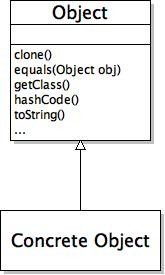
\includegraphics[width=30mm]{img/objectUML.jpeg}
		\caption{Forholdet mellem alle klasser og Objekt klassen  	\label{objectUML}}
	\end{figure}	
	\item Når man \textbf{overrider} en metode i Java betyder det, at man overskriver superklassens version af den pågældende metode
	\begin{itemize}
		\item Når man overrider en metode, må man ikke lave preconditions stærkere,
		\item Man skal også sørger for at overhold \textbf{Lisskovs Substitutions Princip}, som går ud på, at en subklasse af en metode skal kunne bruges samme steder som dens superklasse 
		\item Man skal også sørger for at parameterne er de samme eller overloader man
		\item Returtypen skal enten være den samme type eller en subtype af den pågældende type 
	\end{itemize}
	\item Når man \textbf{overloader} betyder det, at man laver en metode med samme navn som en anden metode dog med anden returtype og/eller parameter. 
	\item Indkapsling er meget vigtig, når man laver et objekt
	\begin{itemize}
		\item Det er god skik, at alle ens felt variabler er private og man tilgår dem kun ved hjælp af getter og setter metoder.
		\item Et immutable objekt er et objekt som når man har instanceret det er det ikke muligt at lave om på det. \textit{Eksempel String objekt} 
	\end{itemize} 
\end{itemize}
	


\subsection{Ligheder og kopiering}
\begin{itemize}
	\item Regler for ligehed i Java:
	\begin{itemize}
		\item Det er reflektivt: x.equals(x) skal altid retunere true
		\item Det er symmetrisk: hvis x.equals(y) er true, så skal y.equals(x) også være true
		\item Det er transtiv: hvis x.equals(y) og y.equals(z) begge retunere true, så skal x.equals(z) også retunere true
		\item For alle reference, der ikke er null skal x.equals(null) altid retunere false
	\end{itemize}
	\item Hashkoder bliver brugt til at definere lighed mellem objekter.
	\begin{itemize}
		\item Alle objekter forskellige fra hinanden skal have forskellige hashkoder.
		\item En hashkode består af en række tal
		\item Fx er hashkode for test strengen \textit{3556498} og test1 \\ strengen \textit{110251487}
	\end{itemize}
	\item Hvis man gerne vil kopier et Java objekt, skal en klasse override metoden clone() og implementere Cloneable interfacet
	\item Clone metoden, som alle objekter nedarver er protected. Derfor kan den ikke tilgået med mindre man overrider den. 
	\item Man kan lave to typer af kopieringer, man kan lave en \textbf{swallow copy} eller en \textbf{deep copy}
	\begin{itemize}
		\item En \textbf{shallow copy} er en kopi, hvor man kun kopier selv elementet og ikke alle elementets feltvariabler (Se figur \ref{shallowCopy})
		\item En \textbf{deep copy} er en kopi, hvor man kopier både selve elementet og alle elementernes feltvariabler, som er objekter. (Se figur \ref{deepCopy})
	\end{itemize}
	\begin{figure}[ht!]
		\centering
		\includegraphics[width=70mm]{img/ShallowCopy.jpeg}
		\caption{Shallow Copy Eksempel\label{shallowCopy}}
	\end{figure}

	\begin{figure}[ht!]
		\centering
		\includegraphics[width=80mm]{img/DeepCopy.jpeg}
		\caption{Deep Copy Eksempel	\label{deepCopy}}
	\end{figure}
	
	\item Hvis man laver en \textbf{Deep Copy} kan man risikere, at der sker et uendelig loop.
	\begin{itemize}
		\item Det kan ske hvis to objekter har en reference til hinanden 
		\item For at undgå dette laver en et check for at undgå at man kopier det samme objekt to gange. 
	\end{itemize}
	\begin{figure}[ht!]
		\centering
		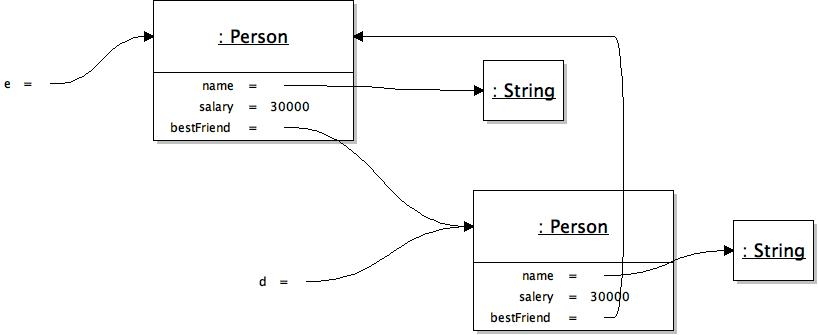
\includegraphics[width=100mm]{img/loopCopy.jpeg}
		\caption{Eksempel på uendelig loop kan forekomme ved kopiering \label{loopCopy}}
	\end{figure}
		
\end{itemize}

\newpage
\subsection{Disposition}
\begin{enumerate}
	\item Javas type system
	\begin{itemize}
		\item Java som type system
		\item Javas typer og værdier
		\item Regler for subtyper i Java
	\end{itemize}
	\item Java objekt model 
	\begin{itemize}
		\item Hvordan er javas objekt model
		\item Overriding og Overloading
		\item Indkapsling
		\item Immutability
	\end{itemize}
	\item Generiske typer
	\begin{itemize}
		\item Hvad er en generisk type?
		\item subtype forholdet
		\item Begrænsning af generiske typer
	\end{itemize}
	\item Lighed og kopiering i Java
	\begin{itemize}
		\item Regler for lighed i Java. 
		\item Hashkoder
		\item Hvordan kopier man i Java?
		\item Shallow copy vs Deep copy
		\item Loop ved kopiering
	\end{itemize}
\end{enumerate}
\newpage

\section{Frameworks and Collections}
\subsection{Frameworks}
\begin{itemize}
	\item Et framework er en samling af klasser og interface typer, som strukturer en mechanisme inde for et bestemt område.
	\begin{itemize}
		\item En programmør kan lave ny funktionalitet framworket ved at udvide frameworkets klasser 
		\item \textit{Et eksempel på dette er Swing frameworket, hvor man kan udvide en Compoment type fx. JFrame eller JCompoment for at lave sin egen Compoment type}
		\item Et framework er ikke et design mønster, men den kan indeholde flere 
	\end{itemize}
	\item En program framework er et framework til at lave applikationer af en bestemt type.
	\begin{itemize}
		\item Et applikations framework har et set af klasser, som en applikations programmør bruger til at lave et applikation ofte ved at udvide de konkrete klasser
		\item I et applikations framework bestemmer frameworkets klasser dens "flow of control" og ikke de applikations specifikke klasser. 
	\end{itemize}
	\item \textbf{\textit{Forskellen på et framework og et biblotek}}
\end{itemize}

\subsection{Java Applets}
\begin{itemize}
	\item En applet er et Java Program, som kører inde i en browser
	\item Java Applets er et simpelt framework.
	\begin{itemize}
		\item Operations kontrol er styret af applet frameworket 
	\end{itemize}
	\item Hvis man vil lave en klasse, som bruger applet frameworket skal den udvide Applet klassen og override nogle af dens metoder
	\begin{itemize}
		\item \textbf{init:} bliver kaldt en gang, når applet først bliver startet.  
		\begin{itemize}
			\item \textbf{Funktion:} at loade alle de grafiske elementer og initialisere data strukturene 
		\end{itemize}
		\item \textbf{start:} Bliver kaldt første gang applet bliver loadet og hver gang at brugeren genåbner browser vinduet der indeholder appleten
		\begin{itemize}
			\item \textbf{Funktion:} Start eller restart inaktive elementer / animationer
		\end{itemize}
		\item \textbf{stop:} Bliver kaldt når brugeren forlader browser windowet eller lukker det
		\begin{itemize}
			\item \textbf{Funktion:} Sørger for at lukke kraftige operationer, når de ikke bruges.
		\end{itemize}
		\item \textbf{destroy:} Bliver kaldt, når browseren bliver lukket
		\begin{itemize}
			\item \textbf{Funktion:} Fjerne alle ressourcer programmet bruger
		\end{itemize}
		\item \textbf{paint:} Kaldes når man skal gentegne vinduet
		\begin{itemize}
			\item \textbf{Funktion:} Gentegn vinduet for at reflektere programmets nuværende tilstand 
		\end{itemize}
	\end{itemize}
	\item Applet Eksempel:
	\begin{itemize}
		\item HTML: 
\begin{lstlisting}[language=html]
<html>
	<body>
		<applet code="AppletEksempel.class" width=230 height=190>
		</applet>
	</body>
</html>
\end{lstlisting}
		\item Java:
\begin{lstlisting}[language=java]
import javax.swing.*;
import java.awt.*;

public class AppletEksempel extends JApplet{
	public void init(){
		setLayout(new FlowLayout());
		add(new JLabel("Hello World!!!"));
	}	
}
\end{lstlisting}
	\end{itemize}
\end{itemize}

\subsection{Collections}
\begin{itemize}
	\item En collection er alle klasser, der på den ene eller anden måde indeholder en samling objekter. 
	\item Alle implementationer af Collections indeholder Genericske typer
	\item Alle collections i collection frameworket implementerer Collection<E> interfacet
	\begin{figure}[ht!]
		\centering
		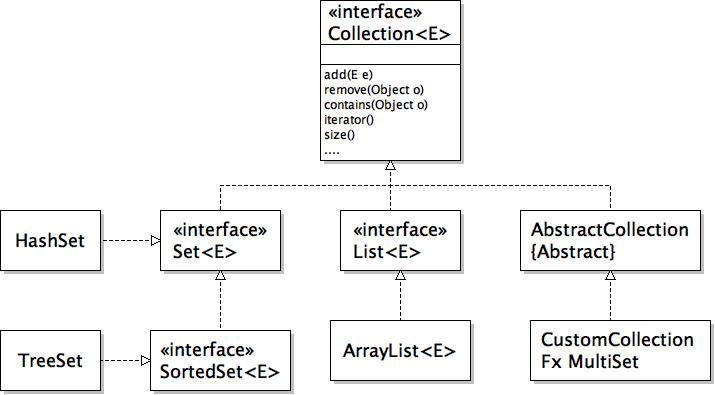
\includegraphics[width=100mm]{img/collectionsUML.jpeg}
		\caption{Collection Framework UML 	\label{UMLCollections}}
	\end{figure}
	\item Der er følgende interface typer i Collection frameworket
	\begin{itemize}
		\item \textbf{Collection:} den mest gennerelle interface type
		\item \textbf{Set:} En collection uden ordre der ikke tillader duplikater
		\item \textbf{SortedSet:} Et set hvis elementer er i sorterede rækkefølge 
		\item \textbf{List:} En ordnede collection .
	\end{itemize}
	\item Eksempler på Collections 
	\begin{itemize}
		\item \textbf{ArrayList:} et alternativ til javas indbyggede arraytype, hvor man kan tilføje uendelig mange elementer
		\item \textbf{HashSet:} et set, som bruger hashkoderne til at lokalisere elementerne. 
	\end{itemize}
	\item Man kan også lave sin egen collection ud fra \textbf{Collection} interfacet.
	\begin{itemize}
		\item Man kan dog også lave en ny collection ud fra \\ \textbf{AbstractCollection}, hvor man kun skal tilføje iterator() og size()
		\item I \textbf{AbstractCollection} behøves man ikke tilføje add() og remove(), de thrower en UnsupportedOperationException hvis de ikke bliver overridet
		\item Multiset Eksempel:

\begin{lstlisting}[language=java]
public class MultiSet <E> extends AbstractCollection<E>{
	private HashMap<E, Integer> _hsm = new HashMap<>();
	private int _size = 0;
	
	public MultiSet(Collection<E> c) {
		addAll(c);
	}
	
	@Override
	public Iterator<E> iterator() {
		return new Iterator<E>() {
			...
		};
	}
	
	
	@Override
	public boolean add(E o) {
		if(_hsm.containsKey(o)){
			int oldValue = _hsm.get(o);
			_hsm.put(o,(oldValue+1));
		}else{
			_hsm.put(o, 1);
		}
			_size += 1;
		return true;
	}
	
	@Override
	public boolean remove(Object o) {
		...
	}
	
	@Override
	public int size() {
		...
	}
	
	@Override
	public boolean equals(Object obj) {
		if(this == obj) return true;
		if(obj == null || getClass() != obj.getClass() ) return false;
		MultiSet multiSet = (MultiSet) obj;
		return multiSet._hsm.equals(_hsm);
	}
}
\end{lstlisting}

	\end{itemize}
\end{itemize}

\newpage
\subsection{Disposition}
\begin{enumerate}
	\item Frameworks
	\begin{itemize}
		\item Hvad er et framework?
		\item Applikations framework
		\item Hvad er forskellen på en framework og et bibliotek?		
	\end{itemize}
	\item Java Applet
	\begin{itemize}
		\item Hvad er en applet og Hvad er formålet?
		\item Eksempel på konceptet \textit{"Don't call us, we call you"} vha. metoder i applet 
	\end{itemize}
	\item Collections
	\begin{itemize}
		\item Hvad er en collection?
		\item Collection Frameworket - UML Diagram
		\item Collection klasser og interfaces
		\item Eksempler + Evt. Multiset Eksempel
	\end{itemize}
	\item Prototype pattern 
	
\end{enumerate}
\newpage

\section{Multithreading}
\subsection{Threads}
\begin{itemize}
	\item En thread er en del af programmet, som bliver kørt uafhængig af andre del af programmet
	\begin{itemize}
		\item Man kan beskrive threads, som små programmer der køre parallelt med hinanden. 
		\item Den vigtige forskel mellem en thread og en process er, at processer ikke kan overskrive hinandens hukommelse, hvorimod threads som køre på en enkelt process godt kan. 
	\end{itemize}
	\item I Java kører Javas virtuel maskine hver thread et kort stykke tid og skifter så til en anden thread.
	\begin{itemize}
		\item Man kan derfor riskerer, at data bliver corrupt, når man bruger flere threads. Derfor er det vigtigt, at tage højte for dette
	\end{itemize}
	\item Thread eksempel Java:
\begin{lstlisting}[language=java]
public class MessageMaker implements Runnable{
	private String _message;
	public MessageMaker(String message){
		_message = message;
	}
	public void run(){
		try{
			System.out.println(_message);
			Thread.sleep(100);
		}catch(InterruptedException e){
		
		}  
	}
}
\end{lstlisting} 

\begin{lstlisting}[language=java]
...
	Thread t1 = new Thread(new MessageMaker("hej"));
	Thread t2 = new Thread(new MessageMaker("farvel"));
	t1.start();
	t2.start();
...
\end{lstlisting}
	\item Hvis man kalder sleep() metoden på Thread klassen sover den pågældende Thread et x andel nanosekunder
	\item En Thread stoppe når dens run metode stopper
	\item Den som sørger for hvilken rækkefølge ens Threads bliver kaldt i bliver kaldt en Time Schuduler 
	\begin{itemize}
		\item Den giver ingen garanti for hvilken rækkefølge ens Threads bliver kaldt i. 
	\end{itemize}
\end{itemize}

\subsection{Thread states}
\begin{itemize}
	\item Alle threads har en tilstand og en prioritet
	\begin{figure}[ht!]
		\centering
		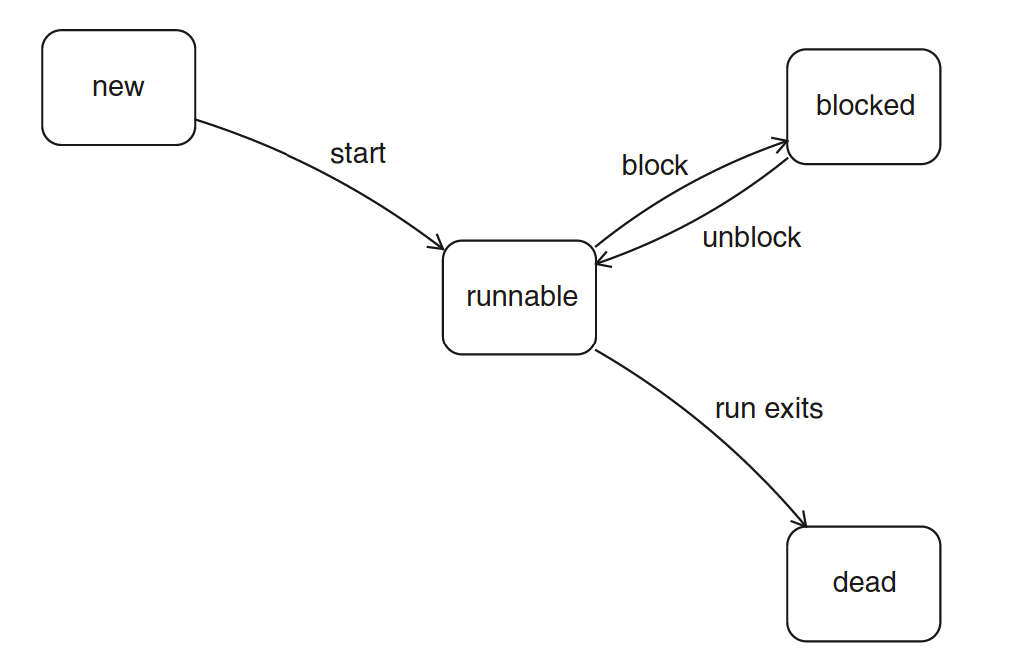
\includegraphics[width=100mm]{img/threadStates.png}
		\caption{Thread States	\label{threadStates}}
	\end{figure}
	\item En threads tilstand er en af følgende:
	\begin{itemize}
		\item Ny (Før start bliver kaldt)
		\item Runnable
		\item Blocked
		\item Dead  når run metoden stopper
	\end{itemize}
	\item Der kan være 4 grunde til at en Thread er blokeret
	\begin{itemize}
		\item Den sover
		\item Venter for input/output
		\item Venter på at få en lås
		\item Venter på en condition
	\end{itemize}
	\item Når en thread er blokeret er den blokeret ind til en bestemt begivenhed forekommer
	\item Thread Schuduleren aktivering en ny Thread, når en af følgende begivenheder forekommer
	\begin{itemize}
		\item En Thread er færdig med dens time slice
		\item En Thread har blokeret sig selv
		\item En Thread med en højre priority er levet runnable
	\end{itemize}
	\item Prioteterne af threadsene afhænger af systemet
	\item For at afbryde en thread skal man kalde interrupt på thread
	\begin{itemize}
		\item Dette afbryder ikke Threaden, den sætte bare en flag, som er Threads egen job at kigge efter.
		\item Det er vigtigt at en Thread kan rydde op efter sig selv
		\item sleep funktionen gør dette af sig selv og smider en interrupted exception, hvis den opdager at den er blevet afbrudt. 
	\end{itemize}
\end{itemize}

\subsection{Thread synchronization}
\begin{itemize}
	\item Når threads de samme objekter kan de konflikte med hinanden
	\item Der komme til at ske en race condition, da thread schuduleren kan stoppe dem midt i at de tilføjer eller fjerner et objekt og derfor kan der ske fejl.
	\item En måde at fixe dette på i Java er ved hjælp af locks. 
	\begin{itemize}
		\item En thread kan accuire en lås også, når en anden Thread prøver at få den samme lås bliver den blocked indtil den anden thread afgiver låsen
	\end{itemize}
	\item Der er 2 slags låse i Java
	\begin{itemize}
		\item Objecter af ReetrantLock klasse eller en anden klasse der implementere lås
		\item Låse som er indbygget i alle Java objekter 
	\end{itemize}
	\item Der kan opstå situationer, hvor der opstår en deadlock, hvor en thread venter på, at en anden thread går noget arbejde. 
	\begin{itemize}
		\item En løsning til en deadlock er at kalde await på en condition, så en anden thread kan få låsen og kalde signal eller signall all på condition, når den er færdig.
	\end{itemize}
	\item Objekt låse:
	\begin{itemize}
		\item Alle jave objeker har en objekt lås
		\item For at beskytte et objekt kan man bruge \textit{"synchronized"} nøgleordet på de metoder man gerne vil beskytte, så får Threadsene automatisk låsene og afgiver dem og man kan kalde wait() og notifyAll() for at bruge conditions. 
	\end{itemize}
	\item Java sync problem:
\begin{lstlisting}[language=java]
public void add(E newValue){
	elements[tail] = newValue;
	tail++;
	size++;
	if(tail==elements.length){
		tail=0;
	}
}
\end{lstlisting}

\begin{lstlisting}[language=java]
..
	private Lock aLock = new ReentrantLock();
	public void add(E newValue){
		aLock.lock();
		try{
			elements[tail] = newValue;
			tail++;
			size++;
			if(tail==elements.length){
				tail=0;
			}
		}finally{
			aLock.unlock();
		}
	}
\end{lstlisting}

\begin{lstlisting}[language=java]
..
	private Lock aLock = new ReentrantLock();
	private Condition spaceAvailableCondition =
	aLock.newCondition();
	public void add(E newValue){
		aLock.lock();
		try{
			while(isFull()){
				spaceAvailableCondition.await();
			}
			elements[tail] = newValue;
			tail++;
			size++;
			if(tail==elements.length){
			tail=0;
		}
		}finally{
			aLock.unlock();
		}
	}
...
\end{lstlisting}

\begin{lstlisting}[language=java]
public E remove(){
	aLock.lock();
	try{
		
		spaceAvailableCondition.signalAll();
		return result;
	}finally{
		aLock.unLock();
	}
}
\end{lstlisting}

	\item java.util.concurrent
	\begin{itemize}
		\item Har en masse formere for collections som automatisk gør brug af locks og conditions
		\item Et godt eksempel er linkedBlockingQueue
		\item Her kan man bruge take() og den blokere automatisk den nuværende thread indtil der kommer noget brugbart. 
	\end{itemize}
\end{itemize}


\newpage
\subsection{Disposition}	
\begin{enumerate}
	\item Threads
	\begin{itemize}
		\item Hvad er en Thread?
		\item Hvordan laver man Threads i Java?
		\item Hvordan stopper man en Thread?
	\end{itemize}
	\item Thread states 
	\begin{itemize}
		\item Hvilke statier kan en thread have
		\item Hvornår kan en thread være blokeret og hvornår vågner den igen?
		\item Hvornår aktiverer thread schedularen en ny thread?
		\item Interrupt()
	\end{itemize}
	\item Thread synchronization
	\begin{itemize}
		\item Raceconditions 
		\item Locks
		\item Conditions
		\item Java bibloteket java.util.concurrent
	\end{itemize} 
\end{enumerate}
\end{document}
%%% Local Variables:
%%% mode: latex
%%% TeX-master: t
%%% End:
